\documentclass[12pt]{article} 
\usepackage[pdftex]{graphicx}
\usepackage{natbib} 
\usepackage{color}
\usepackage{amsmath} 
\usepackage{amssymb} 
\usepackage{verbatim}
\usepackage{mathpazo} 
\usepackage{setspace}
\usepackage{multirow}
\usepackage{fullpage}
\usepackage{lscape}
\usepackage{fancyhdr}
\usepackage[normalem]{ulem} 
\usepackage{hyperref}
\usepackage[parfill]{parskip}
\usepackage{graphicx}
\usepackage{longtable}
\usepackage{times}
\usepackage{textcomp}
\usepackage{xr}
\usepackage{etoolbox}
\usepackage{filecontents}
\usepackage{url}
\externaldocument{SI}
\hypersetup{colorlinks=true, linkcolor=black, citecolor=black}
\RequirePackage{lineno}

\newcommand{\flagged}[1] {
  \textcolor{blue}{#1}
}

\def\title{Major interaction reorganizations punctuate the assembly of
  pollination networks} \def\author{Lauren C.\ Ponisio$^{1,2,3}$,
  Marilia P. Gaiarsa$^4$, Claire Kremen$^1$}

\def\runninghead{Plant-pollinator network assembly}
\def\keywords{community assembly, change points, specialization,
  nestedness, modularity, bipartite, preferential attachment}

\def\extras{
  \begin{itemize}
  \item Submitted as a Letter
  \item Abstract word count: 
  \item Main text word count: 
  \item Number of references: 
  \item Number of figures:
  \end{itemize}
}

\def\affiliation{
  \begin{enumerate}
  \item Department of Environmental Science, Policy, and Management\\
    University of California, Berkeley\\
    130 Mulford Hall\\
    Berkeley, California, USA\\
    94720\\
  \item Berkeley Institute for Data Science (BIDS)\\
    University of California, Berkeley\\
    190 Doe Library \\
    Berkeley, California, USA\\
  \item Department of Entomology\\
    University of California, Riverside\\
    417 Entomology Bldg.\\
    Riverside, California, USA\\
    92521\\
  \item Departamento de Ecologia\\
    Universidade de Sao Paulo\\
    S{\~a}o Paulo, SP, Brazil\\
    05508-900\\
  \end{enumerate}
}

\newcommand{\mstitlepage}{
  \paragraph{Running head:} \textsc{\runninghead}
  % \parindent=0pt
  \begin{center}%
    {\LARGE \title \par}%
    \vskip 3em%
    {\large
      \lineskip .75em%
      \begin{tabular}[t]{c}%
        \author
      \end{tabular}\par}%
    \vskip 1.5em%
  \end{center}\par
  \affiliation
}
\clearpage

\begin{document}

\mstitlepage
\doublespacing
\linenumbers
\clearpage

\begin{abstract}  
  The ability of communities to maintain function in the face of
  species extinction is related to the structure of
  networks. Understanding network structure and how it relates to
  network assembly, therefore, is a priority for conservation
  biology. Using a nine-year-dataset comprising nearly $20,000$
  pollinator visitation records, we explore the assembly of
  plant-pollinator communities at native plant restorations in the
  Central Valley of California. Across years, species are highly
  dynamic in their network position, causing community assembly to be
  punctuated by major interaction reorganizations. In contrast, the
  non-assembling networks did not restructure as frequently. Across
  all communities, pollinator species were opportunistic in the
  flowers they visited. The most persistent and generalized species
  were also the most variable in their network positions, contrary to
  what is expected through prefereantial attachment theory. High
  species and interaction turnover was ubiquitous across assembling
  and non-assembling communities, though unique interactions turned
  over at higher rates in assembling hedgerows as the networks
  continually reorganized. Nestedness of assembling networks also
  increased through time, but there was no increase in robustness to
  simulated plant extinctions. The sensitivity of networks to
  cascading perturbations, however, increased as the communities
  assembled, at least partially due to accumulating species
  richness. We elucidate some of the mechanisms underlying
  plant-pollinator network assembly and restoration, while providing
  further evidence that hedgerows are a valuable tool for promoting
  species conservation and ecosystem service? provision in
  agricultural areas.
\end{abstract}

\keywords

\clearpage

\section*{Introduction}
\label{sec:introduction}

%% introduce mutualisms, restoration, network assembly
Global change has created a severe biodiversity crisis, and as species
are lost, so are their interactions \citep{dunn2009sixth,
  barnosky2011has}. Because mutualistic interactions are essential for
maintaining the diversity of their component guilds, these systems are
particularly at risk from coextinction cascades. The nature of these
cascades will depend on the interaction patterns within a community
\citep{Memmott2004, Rezende2007, Bascompte2009, Thebault2010}. To
safeguard ecological function, it has become increasingly imperative
to aid the recovery of lost interactions and component biodviersity
through ecological restoration, and a key restoration aim is to
facilitate assembly of robust interaction networks
\citep{menz-2010-4}. We know little, however, about how to re-assemble
interacting communities through restoration, or the process of
ecological network assembly more generally.

%% most people think network assemble via preferential attachment, and
%% there is some evidence of that. (other studies on mutualisms?)
Preferential attachment, the most widely explored mechanism of network
assembly, \citep{barabasi1999emergence}, predicts that species
entering a network are more likely to interact with species that are
already well-connected \citep[''the rich-get-richer''
principle,][]{barabasi1999emergence}. In pollination systems --- a
particularly ubiquitous mutualism \citep{ollerton-2011-321,
  klein-2007-303} --- some studies have found support for this
assembly mechanism. Investigating the day-to-day, temporal assembly of
a plant-pollinator network within a season, \cite{Olesen2008} found
that phenologically new plant and pollinator species tended to
interact with already well-connected species, potentially because
these species are either more abundant or more temporally
persistent. In addition, using a space-for-time substitution to study
primary succession along a glacier foreland, \cite{albrecht2010plant}
also found some evidence that assembly occurred through preferential
attachment. Specifically, network nestedness (i.e, a core group of
generalists interacts with both specialist and generalist species)
increased as the community aged \citep{albrecht2010plant}.  An
increase in nestedness could result from the preferential attachment
process where specialist species attach to the well-connected,
generalist core.

%% there are other ways to assemble that are not preferentia;
%% attchment, particularly vis big reorganizations of interactions
%% Lauren I love this paragraph!
In contrast to the network build-up described by preferential
attachment, significant reorganizations of interactions can punctuate
assembly \citep{peel2014detecting}. Such significant reorganizations
of interactions, or network changing points, are observed in social
networks that respond to abrupt shifts in the behavior of interactors
\citep{peel2014detecting}. In ecological communities, such shifts may
occur if, as new species colonize, resident species change their
interaction partners to optimize their foraging effort. In
plant-pollinator communities, theory predicts that pollinators
optimize their use of floral resources to reduce interspecific
competition and improve resource-use efficiency
\citep{pyke1984optimal, valdovinos2010consequences,
  valdovinos2013adaptive, albrecht2010plant, Bluthgen2007}. No
studies, however, have examined whether network changing points occur
during ecological network assembly, and how these changes relate to
the species behavior.

%% restoration
Understanding network assembly is particularly relevant to ecological
restoration, which is essentially 'applied succession'
\citep[e.g.,][]{parker1997scale}. In pollination systems, the time
since an area was restored has been shown to affect the structure of
networks \citep{forup-2008-742, devoto2012understanding}, suggesting
interactions are changing as the community develops. Understanding the
mechanisms of network assembly will help to guide community
restoration. Facilitating network restoration is especially imperative
in areas where species interactions provide essential ecosystem
services, such as crop pollination. To ensure the continued provision
of ecosystem services and curb biodiversity loss, it is critical to
restore pollinators and their interactions in agricultural
landscapes. To promote pollinator services in agriculture, farmers may
chose to plant strips of native plants along farm edges (hedgerows) to
help provide habitat for pollinators without removing arable land from
production. Hedgerows augment the richness, abundance and trait
diversity of pollinators in agricultural landscapes
\citep{morandin-2013-829, kremen-2015-602, ponisio2015farm}, and
promote the persistence and colonization of floral resource
specialists \citep{mgonigle-2015-x}. It is important to understand how
these new species are being incorporated into the network as the
community assembles, and the consequences for interaction patterns and
robustness.

%% Lauren I would put 10 year dataset; and I *loved* the way you
%% organized the ideas here!!
We explore the process of network development using a nine year
dataset of plant-pollinator community assembly following hedgerow
restoration in the highly simplified and intensively managed
agricultural landscape of California's Central Valley.  We first
determine whether the mechanism underlying network assembly is a build
up of interactions as would be predicted by preferential attachment,
or instead is punctuated by significant reorganizations of
interactions (i.e., network changing points). Even with changing
points in interaction organization, networks could still be assembling
via preferential attachment if the network reorganizations were
primarily driven by peripheral, temporally variable species while a
stable, well-connected core of species persist. We test whether the
species that are most variable in their network position --- and thus
important contributors to network reorganizations --- are less
persistent and connected species. To further explore the mechanisms
underlying the temporal dynamics of the networks, we examine patterns
in the species and interaction temporal turnover. Lastly, we
investigate whether networks are assembling toward predictable
interaction patterns, and the ramifications for the robustness of the
networks to species extinction and cascading perturbations.

%% objectives
% 1) Are hedgerows assembling by preferential attachment, or are there
% more abrupt reorganizations of network structure?
% 2) Who are the species responsible for interaction reorganizations?
% how to incorporate this? 
% 3) Are the changing points a product of turnover in species
% composition, or are more substantial changes in the verticles of the
% networks?
% 4) Is the structure of interactions changing? Does this change the
% robustness of the network to species extinction and/or perturbation?

\section*{Materials \& Methods}
\label{sec:methods}

\subsection*{Study sites and collection methods}
\label{sec:study-sites}

We surveyed plant-pollinator interaction networks of independent
assembling hedgerows communities (N=5), and of two types of
non-assembling communities to serve as controls: unrestored, weedy
field margins (N=19) and mature hedgerows (greater than 10 years since
planting, N=29). The sites were located in the Central Valley of
California in Yolo, Colusa and Solano Counties. This area is composed
of intensively managed agriculture --- primarily monocultures of
conventional row crops, vineyards and orchards. Hedgerows are ca.~3--6
m wide and approximately 350 m long, bordering large (ca.\
30--hectare) crop fields. Hedgerows consist of native, perennial,
shrub and tree plantings including \textit{Rosa californica},
\textit{Cercis occidentalis}, \textit{Ceanothus spp.},
\textit{Heteromeles arbutifolia}, \textit{Sambucus mexicana},
\textit{Eriogonum spp.}, \textit{Baccharis spp.}, \textit{Salvia
  spp}. and others \citep[Fig.~S1][]{menz-2010-4, kremen-2015-602,
  mgonigle-2015-x}. The mean distance between monitoring sites was
$15$ km, and the minimum distance between sites sampled in the same
year was 1 km.  The entire area surveyed spanned almost $300$
km$^2$. The crop fields adjacent to all sites were similarly managed
as intensive, high-input monoculture.

Monitoring of assembling hedgerows began in 2006 and continued through
2014. Surveys of these sites began the year before the area was
restored. For logistical reasons, no sampling of assembling hedgerows
was conducted in 2010. Sites were sampled between two and five times
per year (Tables S1-S3, mean $3.4$ samples per year). In each round of
sampling, the order in which sites were sampled was
randomized. Surveys were conducted under sunny conditions when the
temperature was above $21^{\circ}\mathrm{C}$ and wind speed was below
$2.5$ meters/second.

Flower-visitors to plants in hedgerows and unrestored controls were
netted for one hour of active search time (the timer was paused when
handling specimens). Honeybees (\textit{Apis mellifera}) were not
collected because their abundance is determined largely by hive
placement by bee-keepers. All other insect flower visitors that
touched the reproductive parts of the flower were collected; however,
here we focus only on wild bees and syrphids --- the most abundant and
effective pollinators in the system (representing 49 and 19 percent of
records, respectively, C.~Kremen, A.~Klein and L.~Morandin,
unpublished data). Bee and syrphid specimens were identified to
species (or morpho-species for some bee specimens in the genera
\textit{Nomada} and \textit{Sphecodes}) by expert taxonomists.

Quantitative networks were generated for each site through time. To
account for the unequal number of surveys between years (Tables
S1-S3), we use the mean of the interactions between a pair of plants
and pollinators across surveys within a year to represent interaction
frequency.

\subsection*{Change point analysis}
\subsubsection*{Identifying change points}
We employed a change point detection method \citep{peel2014detecting}
to identify fundamental reorganizations in large-scale interaction
patterns. A change point is caused by a merge, split, fragmentation or
formation of modules (also called compartments). Change point
detection methods have yet to be generalized to quantitative networks,
so for this analysis we focused on qualitative (binary)
networks. Following \cite{peel2014detecting}, we first defined a
probability distribution over the networks using the generalized
hierarchical random graph model (GHRG). The GHRG model is able to
capture both assortative and disassortative structure patterns at all
scales in the network \citep{peel2014detecting}. A network $G$ is
composed of vertices $V$ and edges $E$. The GHRG model decomposes the
$N$ vertices into a series of nested groups, the relationships among
which are represented by the dendrogram $T$. The tips of $T$ are the
vertices of $G$, and the probability that two vertices $u$ and $v$
connect is given by the parameter $p_r$. The probability distribution
of the network $G$ is thus defined as:

\begin{equation}
  \label{eq:lik}
  P(G|T,{pr}) = p_r^{E_r}(1-p_r)^{N_r-E_r}
\end{equation}
% 
Where $E_r$ is the observed number of edges between vertices with the
common ancestor $r$, and $N_r$ is the total possible edges.

Using Bayesian posterior inference and techniques from phylogenetic
tree reconstruction, we fit the GHRG model to the networks
\citep{peel2014detecting}. This is accomplished by using a Markov
chain Monte Carlo (MCMC) procedure to first sample the posterior
distribution of bipartitions, from which a consensus tree is derived
\citep{peel2014detecting}. We use $\beta$ distributions with the
hyperparameters $\alpha=\beta=1$ to define priors for $p_r$.

Once the GHRG model has been fit to the networks, we determine whether
a change point occurred between two time slices. To detect a change
point, we use Bayes factors to compare the fit of two models --- one
where a change point occurred between two networks, and one where no
change occurred. We chose a sliding window of length, $w$, of four,
within which to find change points. Larger windows allow for more
gradual changes, and four was the maximum possible with our eight
years of data. Lastly, to calculate a $p$-value for the Bayes factors,
we use parametric bootstrapping to numerically estimate the null
distribution \citep{peel2014detecting}. We employed code published
online by L.~Peel for the change point analysis. Analyses were
conducted in Python 3.4.

We next test whether the change points occurring in maturing hedgerows
were a component of the assembly process or a product of environmental
shifts that lead to network reorganizations in all types of
communities. We model the number of change points as successes and the
total number of years each site was sampled as trials, and use a
generalized linear model with Binomial error to test whether the
probability of a change point occurring varied by site type. We used
standard techniques to determine whether the assumptions of the models
were met for this and all subsequent models. For the non-assembling
hedgerows and weedy field margins, only sites with five or greater
survey years were included in this analysis (N=11). All statistical
analyses were conducted in R 3.2.3 \citep{R}.

\subsubsection*{Characteristics of species that contribute to change
  points}

To further elucidate the nature of the change points, we examine the
characteristics of the species that contributed to interaction
reorganization. Some species remain in relatively similar network
positions through time, whereas others are more variable in their
position and thus contribute more strongly to network
reorganization. We test whether the more persistent species with the
highest degree (number of different interaction partners) are the
most stable in their network positions, as would be expected if the
networks were assembling via preferential attachment.

We calculate species persistence as the proportion of surveys in which
a plant or pollinator is observed. Species observed consistently
within and between years are thus maximally persistent. Weighted
species degree is calculated from interaction observations from an
extensive dataset from Yolo County (approx.~18000 interaction records)
that included both the data included in this study and additional data
from sites where we collected flower visitors using the same methods
\citep{mgonigle-2015-x, ponisio2015farm}. To represent network
position variability, we computed the coefficient of variation of
weighted closeness centrality \citep{freeman1978centrality} at each
site through time. Closeness centrality represents the importance of a
space by calcuating the path lengths to other vertices (species) in
the network \citep{freeman1978centrality}. The shorter the mean path
length to other species, the higher is the closeness centrality. We
use linear mixed models to test whether the species closeness
variability (log) is related to the persistence or degree of that
species \citep{lme4, lmetest}. We included random effects for species
and site. Because the degree and persistence of pollinators were
strongly correlated, ($\rho = 0.84$, $p$-value $<$ $2*10^{-16}$), we
include each explanatory variable in separate models. Plant degree and
persistence were not significantly correlated, but we use the same
models as we did for the pollinators for consistency.  Because an
approximately logarithmic increase in closeness centrality, as would
be expected with assembly by preferential attachment, would also lead
to high variability in closeness scores, we also test whether log
closeness centrality increases through time.

\subsection*{Species and interaction turnover}

%%Lauren I really liked the way you explained this part =]
Reorganizations of network structure can be the result of species
turnover or species changing their interaction partners (i.e.,
re-wiring). To better understand the mechanisms underlying the
temporal dynamics of the assembling networks, we examined patterns of
species and interaction turnover. For example, assembling networks may
have higher rates of pollinator turnover than non-assembling
communities because new pollinator species are colonizing and
establishing themselves \citep{mgonigle-2015-x}. Similarly, because
species are turning over and pollinators are trying to maximize their
foraging efficiency based on the species present, interactions may
turnover more quickly than in established communities. In addition, at
assembling hedgerows, plants that are unvisited in early years may
appear to ``colonize'' the networks as they became more attractive
resources and establish new interactions with pollinators.

To estimate the temporal species and interaction turnover, we use an
approach similar to calculating spatial $\beta$-diversity. Instead of
calculating the variation in community composition across sites within
a year, we estimated turnover across years at a site. We first
calculated the pairwise dissimilarity of plants, pollinators and
interactions between years within each site using the Chao
dissimilarity estimator that incorporates abundances, while also
accounting for unobserved records \citep{chao-2005-148}. Dissimilarity
estimates can be affected by the total number of species and
individuals sampled at a site \citep[e.g.,][]{ponisio2015farm}. For
example, the probability that two sites do not share any species is
higher when there are few individuals at those sites. Following
\cite{ponisio2015farm}, we use null models that constrained species
richness to estimate the deviation of the observed dissimilarity from
that which would be expected under a random community assembly
process. With the corrected dissimilarity values, we then calculated
the multivariate dispersion of community composition across years
\citep{anderson-2011-19}. In order to test whether assembling
hedgerows had more species and interactions turnover than
non-assembling communities, the species and interaction temporal
turnover estimates were modeled as responses in a linear mixed model
with site type as an explanatory variable and site as a random effect
\citep{lme4, lmetest}.

Though species may turnover across years, some groups of species may
essentially replace each other if they fill similar roles in the
network, occupying the same network position and interacting with
similar species. At non-assembling communities, species turnover may
overestimate the temporal changes in the networks if the interactions
occurring in one year are similar to those in the next year when they
are weighted by the similarity of their constituent species
(Fig.~\ref{fig:methods}). We develop a method to examine the temporal
turnover of interactions with weightings based on their similarity. We
followed the algorithm of \cite{ahn2010link} to cluster all the
interactions (edges) hierarchically across sites and years based on
their similarity, and build a dendrogram. The interaction similarity
is based how may plants and pollinators (vertices) two edges share
\citep{ahn2010link, kalinka2011linkcomm}. The more species edges
shared in common, the shorter the branch length between them on the
dendrogram.  We next calculated the temporal turnover of interactions
weighted by their similarity, as approximated by ``phylogenetic''
distance \citep{graham2008phylogenetic, picante-2010-1463}. We then
use linear models to test whether the weighted turnover of
interactions varied between assembling and non-assembling networks
\citep{lme4, lmetest}.

\section*{Temporal changes in interaction patterns}

\subsection*{Network structure}
Any changing points in network structure may contribute to the
reorganization of the assembling networks into predictable interaction
patterns. Pollination networks exhibit two main structural patterns
--- modularity \citep[e.g.,][]{Olesen2007} and nestedness
\citep[e.g.,][]{Bascompte2006, Bascompte2003}. In modular networks,
interactions are insular, occurring within separate groups or
``modules'' more often than between modules. Modules in the network
may fragment as the network assembles, enhancing
modularity. Conversely, nested networks are like a pyramid of
interactions, where there are some species that interact with many
species, other species that interact with a subset of those species,
and so on. If species entering the network tend to interact with the
generalist base of the network pyramid as would be expected with
preferential attachment, nestedness would increase through time. The
connectance --- the proportion of observed out of possible
interactions --- would decrease as new, specialist species,
preferentially attach to the core.  Lastly, the overall level of
network specialization may change as the community
assembles. Network-level specialization will increase if specialist
species colonize the network or species begin to limit their
interaction niche breath as the network assembles
\citep{bluthgen-2006-9}.

To evaluate network nestedness, we used the estimator weighted NODF
\citep{almeida-neto-2008-1227}. NODF evaluates whether species with
fewer partners interact with subsets of partners with which more
connected species interact \citep{almeida-neto-2008-1227}. To estimate
modularity, we use a hierarchical clustering algorithm
\citep{Newman2004, csardi-2006}. We evaluate network specialization with
the metric H2, which estimates the deviation of the observed
interaction frequency between plants and pollinators from a null
expectation where all partners interact in proportion to their
abundances \citep{bluthgen-2006-9}. It ranges from zero for
generalized networks to one for specialized networks.  We calculated
standardized $z$-scores so that nestedness, modularity and
specialization metrics could be compared across communities. The
$z$-scores were calculated by generating an ensemble of $999$ randomly
assembled communities, subtracting the mean of the statistic
calculated across these communities from the observed value, and then
dividing by the standard deviation. To assemble random communities, we
reshuffled the interactions between species but fixed the total number
of interactions, species and interaction frequency distributions
\citep{Galeano2009}.

To test whether network modularity, nestedness, connectance or
specialization changed linearly with assembly, we used linear mixed
models with the descriptive network metrics as the response variable,
year of assembly as the explanatory variable, and random effects of
site and year. The number of species in a network affects the patterns
of interaction possible, so we also examined the change in plant and
pollinator species richness through time. We employ generalized linear
mixed models with Poisson error to model richness. We scaled
explanatory variables.


\subsection*{Network robustness}
Lastly, we tested whether the changes in interaction patterns
associated with network assembly affect the robustness of the network
to species loss and cascading perturbations. Following
\cite{Memmott2004}, we simulated plant species extinction and the
subsequent extinction cascades of pollinator species. Because the
reproduction of plant species is facilitated by active restoration
efforts, it is unlikely the extinction of pollinator species would
affect plant populations in the hedgerows. However, plants ceasing to
bloom, for example in response to drought, will likely affect the
pollinators that depend on them. We eliminated plants species based on
their degree or abundance, and then calculated the number of
pollinators that secondarily went extinct. The area below the
extinction curve is an estimate of network robustness
\citep{Memmott2004, bipartite}.

We also explored how the robustness to cascading perturbations changed
as the community assembled, using algebraic connectivity --- the
second smallest eigenvalue of the Laplacian matrix
\citep{fiedler1973algebraic} --- as a proxy for network robustness
(Gaiarsa et al., in prep). Algebraic connectivity relates to how
difficult it is to turn a network into completely disconnected groups
of species \citep{costa2007characterization, gibert2013spatial}. The
larger the algebraic connectivity, the more sensitive a network is to
cascading perturbations. Perturbations, such as the decrease in abundance of a
plant or pollinator, can have negative consequences
for the species in the network. For example, pollination service provided to planst could decrease following a decrease in
abundance of a pollinator. The affected plants would set less seeds,
and decrease in abundance the subsequent year. Consequently, other pollinators that
depended on those plant species would also be affected, and the effects of this perturbation would
continue to propagate throughout the network, potentially affecting all species in the community. Alternatively, perturbations could
also have a positive effect. For example, the increase in abundance of a
plant species would lead to an increase in resource availability for the pollinators. The examples
of negative perturbations (e.g., resource collapse, disease spreading,
parasites), however, outnumber possible positive perturbations. It is important to point out that both robustness and algebraic connectivity assume that the network is static --- these metrics do not
account for the ability of species to alter their interaction
depending on circumstances and the resource availability.

\section*{Results}
\label{sec:results}

Over eight years and $747$ samples, we collected and identified
$19,547$ wild bees and syrphids comprising $173$ species from $50$
genera. We observed $1,521$ unique interactions between plants and
pollinators.

\subsection*{Change point analysis}
\subsubsection*{Identifying change points}

The majority ($76\%$) of the sites underwent at least one significant
interaction reorganization (Fig.~\ref{fig:changePoints},
\ref{fig:changePoints2}).  All five of the assembling hedgerows
experienced network changing points, whereas only $40\%$ and $81\%$ of
non-assembling hedgerows and field margins, respectively, underwent
significant interaction reorganizations. Assembling hedgerows had
significantly more changing points than the non-assembling networks
(estimate of the difference in the odds ratios between assembling and
non-assembling networks, $3.316$, $95\%$ CI $[1.314, 8.572]$,
$p$-value= $0.0117$). Network assembly following restoration is thus
punctuated by more interaction reorganizations than would be expected
by environmental shifts alone that would effect all networks
similarly.

\subsubsection*{Characteristics of species that contribute to change
  points}

In contradiction to the predictions of assembly by preferential
attachment, both pollinator persistence and degree were positively
related to network position variability (Fig.~\ref{fig:cv}, estimate
of the slope of closeness centrality variability and persistence $\pm$
standard error of the estimate, $0.653 \pm 0.225$, $p$-value=$0.009$;
slope of closeness centrality variability and degree, $0.008 \pm
0.002$, $p$-value=$0.002$). The slope of these relationships remained
significant when the species with the top $10$ persistence and degree
scores were dropped. In addition, plant persistence and degree were
not significantly related to network position variability
(Fig.~\ref{fig:cv}). % estimate of the slope of closeness variability and
% persistence $\pm$ SE, $-2.063 \pm 3.091$, $p$-value=$0.5$; slope of
% closeness variability and degree, $0.0018 \pm 0.002$,
% $p$-value=$0.3$).
The variability of species network position was not the result of
closeness linearly increasing through time, and, in fact, plant and
pollinator closeness decreased slightly through time (Fig.~S2,
estimate of the slope of closeness through time $\pm$ SE, pollinators:
$-0.0003 \pm 0.00005$, $p$-value=$2.7*10^{-12}$; plants $-0.007 \pm
0.001$, $p$-value=$1.4*10^{-6}$). Through statistically significant,
the slopes are so slight they may not be biologically significant.

\subsection*{Species and interaction turnover}
The rates of plant, pollinator and interaction temporal turnover were
similar across assembling hedgerows, non-assembling hedgerows and
field margins, though mature hedgerows has marginally significantly
less pollinator turnover than field margins (Fig.~\ref{fig:beta},
estimate $\pm$ SE of the difference in
turnover between field margins and mature hedgerows, $-0.0498 \pm
0.026$, $p$-value=$0.058$). When interactions where weighted by their
similarity, both assembling and mature hedgerows had higher rates of
turnover than field margins (Fig.~\ref{fig:beta}, estimate $\pm$
SE of the difference in turnover between
field margins and assembling hedgerows, $0.115 \pm 0.027$,
$p$-value=$0.0002$; field margins and mature hedgerows, $0.082 \pm
0.024$, $p$-value=$0.002$). The weighted interaction turnover at
assembling hedgerows, however, was not significantly higher than in
non-assembling, mature hedgerows.

\section*{Temporal changes in interaction patterns}
\subsection*{Network structure}
Network nestedness significantly increased with assembly
(Fig.~\ref{fig:baci}, estimate of the slope of nestedness through time
$\pm$ SE, $1.834 \pm 0.6142$, $p$-value=$0.022$). All of the networks
were significantly nested ($z$-scores $>$ 2,
Fig.~\ref{fig:baci}). Modularity decreased (Fig.~\ref{fig:baci}),
though the slope was not significantly different from
zero. % (estimate
% of the slope of modularity through time $\pm$ standard error of the
% estimate, $-0.524$ $\pm$ $0.295$, $p$-value=$0.124$).
In addition, none of the networks were significantly modular
($z$-scores $<$ 2, Fig.~\ref{fig:baci}). Connectance decreased as the
community assembled (Fig.~\ref{fig:baci}, estimate of the slope of
connectance through time $\pm$ standard error of the estimate,
$-0.0434$ $\pm$ $0.0152$, $p$-value=$0.03$). Specialization also
decreased, though the slope was only marginally significantly
different from zero (estimate of the slope of specialization through
time $\pm$ SE, $-0.926$ $\pm$ $0.450$, $p$-value=$0.078$). Most
communities were more generalized than expected when interactions were
randomized (Fig.~\ref{fig:baci}).

Both plant and pollinator species richness increased through time
(Fig.~\ref{fig:baci}, estimate of the slope of richness through time
$\pm$ SE, pollinators: $0.193$ $\pm$ $0.0729$, $p$-value=$0.008$;
plants: $0.212$ $\pm$ $0.0653$, $p$-value=$0.001$). Unsurprisingly,
pollinator species are colonizing and persisting at the assembling
hedgerows. Plant species richness in the networks is based on the
flowers actually visited by pollinators and not the presence of a
particular plant species at a site. Thus, though some new plant
species may establish themselves in the hedgerows, the increase in
plant richness in the networks is likely due to previously unvisited
plants attracting visitors as they mature and offer better rewards.

\subsection*{Network robustness}
Assembly did not effect the robustness of the networks to species
extinction when species were removed incrementally by
degree % (estimate
% of the slope of robustness through time $\pm$ SE, $6*10^{-5} \pm
% 4*10^{-3}$, $p$-value=$0.987$)
or abundance. % ($0.001 \pm 0.003$,
% $p$-value=$0.65$)
In contrast, the sensitivity of networks to
cascading perturbations, as measured by the algebraic connectivity of
the network, increased as the network assembled (Fig.~\ref{fig:rob},
estimate of the slope of sensitivity to cascading perturbations
through time $\pm$ SE, $0.6814 \pm 0.272$, $p$-value=$0.042$).

\section*{Discussion}
\label{sec:discussion}

We show that the temporal assembly of plant-pollinator networks
following restoration is a highly dynamic process where interactions
often undergo significant reorganizations, the so called changing
points. If these network reorganizations were a product of
environmental forces alone, we would expect to observe the same
changing points at the same periods, consistently across all
sites. However, network changing points in non-assembling communities
are less frequent, and there are few consistent trends in when change
points occurred across all sites. Several sites had network changing
points between years 2009 and 2011 (Fig.~\ref{fig:changePoints}). In
California, 2011 marked the beginning of a multi-year drought. The
assembling hedgerows were not sampled in 2010, so disentangling
whether the changing points are due to skipping a year of monitoring
the assembly process or the drought is not possible. Interestingly,
most assembling hedgerows did not undergo a significant interaction
reorganization immediately after a hedgerow was planted (i.e., the
transition from weedy field margin to hedgerow). This result is
consistent with the finding that in our study system, hedgerow
restoration takes several years to have an impact on the
plant-pollinator communities, and with the observation that hedgerows
do not begin to produce many flowers until $3$--$5$ years following
planting (Kremen and M'Gonigle, in prep).

In addition to finding multiple network organization changing points
during assembly, the way in which these reorganizations occur was
different from what would be expected from preferential
attachment. With a preferential attachment process, we expect that the
most persistent and high degree species would remain stable in the
network core during assembly
\citep{barabasi1999emergence}. Surprisingly, however, we encountered
the opposite pattern. For example, the four most ubiquitous species in
our study landscape --- \textit{Halictus ligatus}, \textit{Halictus
  tripartitus}, \textit{Lasioglossum (Dialictus) incompletum}, and
\textit{Toxomerus marginatus} --- were the only species that changed
which module they were a member in across years in all the assembling
hedgerows. Because species degree and persistence were strongly
correlated, it is difficult to disentangle the causal mechanism for
why species with those characteristics are so variable in their
network position. Generalized species may be better able to exploit
the limited floral resources in the intensively managed agriculture
landscape, and thus also be the most persistent \citep[in ant-plant
mutualisms, ][]{diaz2010changes}. More persistent species usually have
longer phenologies, so they can visit many different flowers,
resulting in a higher degree \citep{Vazquez2009,
  fort2016abundance}. Either way, our result suggests that adaptable
species can change their network position to utilize the most
advantageous floral resources available, which may depend on both the
other pollinator species that are present and the state of the plant
community \citep{macleod2016measuring, gomez2006ecological,
  Waser1996}. Thus given the opportunity and ability to
use different resources, species will often change their network
positions \citep{macleod2016measuring}.

Interestingly, though assembling hedgerows had more network
reorganizations than non-assembling communities, pollinator species
and interaction turnover occurred at similar rates across site types.
Assembling hedgerows have higher turnover than non-assembling field
margins only when interactions were weighted by their similarity. This
is likely because though species and interactions are turning over at
the field margins, species and interactions that fill similar roles in
the network are replacing each other. In contrast, at the assembling
hedgerows, unique interactions are turning over as the networks
continually reorganize. Non-assembling mature hedgerow communities,
however, had similar rates of weighted interaction turnover as
assembling hedgerows but also the lowest pollinator
turnover. Pollinator communities at mature hedgerows may be generally
more stable, but rare and/or specialized pollinators could generate
this pattern if they entered a community, formed unique interactions
with plants that did not previously share pollinators, but did not
persist in the networks. These species would not contribute strongly
to network reorganization or species turnover, but would enhance
weighted interaction turnover. Mature hedgerows may thus both support
more stable pollinator communities, while also providing resources for
rare and/or specialized species \citep{kremen-2015-602,
  mgonigle-2015-x}.

When we explore the how network-level interaction patterns changed
through time, we found that nestedness did increase as the community
assembled, as would be expected if colonizing, specialist species
preferentially attached to a central, generalist core
\citep{albrecht2010plant}. In addition, connectance decreased, as
would be expected if the network is being colonized by specialist
species and the overall mean number of interactions per species did
not change. However, the frequent changing points in network
organization, dynamic nature of species positions in the networks, and
turnover of species and interactions all point to an assembly
mechanism other than preferential attachment.  The stable level of
network-level specialization through the assembly process may be due
to the increased colonization of specialized species
\citep{mgonigle-2015-x} accompanied by an increase in the diet breath
of resident species. This would be expected if resident species were
able to minimize their foraging time by expanding their diet breath as
plant diversity increases with hedgerow maturation \citep{Waser1996,
  pyke1984optimal, Bluthgen2007, albrecht2010plant}. Such a change in
pollinator behavior would also explain the increase in network
nestedness. Because so many mechanisms give rise to the same patterns
of interaction, additional tests are necessary to assess the
contribution of different mechanisms to community assembly.

Interestingly, however, the changes in network patterns associated
with assembly did not effect the robustness of hedgerow communities to
species loss. This is particularly surprising given the observed
increase in nestedness, which is often associated with an enhanced in
robustness to extinction \citep{Memmott2004}. Perhaps assembling
hedgerows have yet to reach sufficient levels of nestedness to realize
the benefits nestedness confers. Nestedness of the assembling
hedgerows, however, did not asymptote within the eight years following
restoration that the sites were surveyed, so hedgerow networks may
eventually reach sufficient levels of nestedness to gain the
robustness advantage.

Contrary to the general restoration goals, the susceptibility of the
networks to cascading perturbations increased as the communities
assembled. Because network vulnerability to cascading perturbations,
as measured by algebraic connectivity, is correlated with species
richness, the increase in and plant and pollinator richness following
restoration is at least partially responsible for the increase in
response to cascading effects. Connectance is also positively related
to algebraic connectivity \citep{gibert2013spatial}, but because we
observed a decrease in connectance, topological characteristics of the
networks beyond species richness and connectance are needed to explain
the increased sensitivity to perturbations spreading. These hedgerows
were designed to provide floral resources to the largest number of
pollinators across the growing season \citep{menz-2010-4}. The
generalized nature of the floral community may explain why the
networks tended to be more generalized than expected if interactions
were randomly distributed across species (Fig.~\ref{fig:baci}). In
addition, the design of the hedgerow plantings may have facilitated
the emergence of a single, highly connected module in all of the
networks (see \ref{fig:changePoints2} for examples). This network
configuration results in short path lengths (the distance between
species in a network based on their shared partners), and thus, a
perturbation in one species can more easily spread to other
species. In order to promote more resilient communities, future
restoration efforts should explore designing floral communities to
promote more interaction partitioning using, for example, algorithms
to optimize different network properties based on prior knowledge of
pollinator floral preferences \citep{mgonigle2016tool}, and on desired
network architectures that renders them more robust both to species
loss and to cascading effects.


% The relationship between diversity and stability in networks
% has been the subject of considerable debate
% \citep[e.g.,][]{may1972will, pimm1984complexity,
%   montoya2006ecological}. Our results provide one of the few empirical
% examples of how restoring species diversity contributes to enhancing
% network stability.

% providing further evidence that hedgerows are a valuable tool for
% promoting species conservation and ecosystem provision in agricultural
% areas \citep{mgonigle-2015-x, ponisio2015farm,
%   kremen-2015-602}.

Plant-pollinator networks, in general, are highly dynamic, with high
turnover of species and interactions both within and between seasons
\citep{Burkle2011}. Though our non-assembling communities experience
fewer network reorganizations than the assembling hedgerows, $82\%$ of
field margins and $40\%$ of mature hedgerows underwent at least one
changing point in network structure. Pollinators are also highly
opportunistic \citep{petanidou-2008-564, Vazquez2005b,
  albrecht2010plant}, though trait complementarity such as tongue
length and corolla depth impose some biophysical limits to the
interactions between plants and pollinators
\citep{Vazquez2009evaluating, Vazquez2009, Stang2009, Stang2006,
  Santamaria2007}. Such opportunism may buffer plant-pollinator
communities from global change \citep[e.g.,][]{ramos2012topological,
  kaiser2010robustness}, but our limited understanding of the assembly
of these communities impedes making such predictions
\citep{Vazquez2009, Burkle2011}. Unlike in the broader food web
literature, we have few assembly models of mutualistic network
assembly \citep{valdovinos2013adaptive, Nuismer2013, Guimaraes2011}.
In addition, the few developed models often borrow their mechanisms
from competitive interactions, leading to inaccurate biological
assumptions \citep{holland2006comment}. We need further development of
mechanistic models of mutualistic systems to generate testable
predictions, along with empirical exploration of network
assembly. Plant-pollinator communities and mutualisms broadly are
vital for biodiversity maintenance and essential ecosystem service
provision. We must therefore understand the processes underlying their
assembly to facilitate restoration and conservation.

\section*{Acknowledgments}
\label{sec:acknowledge}

We would like to thank Paulo R.~Guimar{\~a}es Jr., Aaron Clauset and
Matthew Hutchinson for their invaluable discussions and comments, and
Leto Peel for help with the change point analysis.  We thank the
growers and land owners that allowed us to work on their property. We
also greatly appreciate the identification assistance of expert
taxonomists Martin Hauser, Robbin Thorp and Jason Gibbs.  This work
was supported by funding from the Army Research Office
(W911NF-11-1-0361 to CK), the Natural Resources Conservation Service
(CIG-69-3A75-12-253, CIG-69-3A75-9-142, CIG-68-9104-6-101 and
WLF-69-7482-6-277 to The Xerces Society), the National Science
Foundation (DEB-0919128 to CK), The U.S.  Department of Agriculture
(USDA-NIFA 2012-51181-20105 to Michigan State University).  Funding
for LCP was provided by an NSF Graduate Research Fellowship, the USDA
NIFA Graduate Fellowship, and the Berkeley Institute for Data
Science. Funding for MPG was provided by S{\~a}o Paulo Research
Foundation (FAPESP, grant 2013/13319-5). We also appreciate the Santa
Fe Institute for facilitating this international collaboration.

\bibliographystyle{ecol_let}

\bibliography{refs}

\clearpage
\begin{figure}
  \centering
  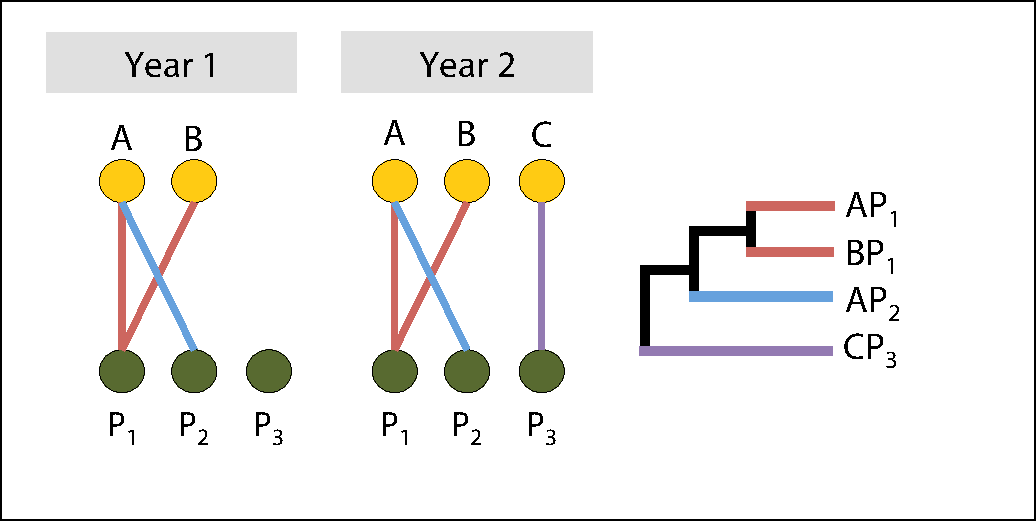
\includegraphics[width=.8\textwidth]{figures/scheme.pdf}
  \caption{Diagram illustrating the analysis to examine the temporal
    turnover of interactions weighted based on their similarity. A, B
    and C are animal species, and Ps are plant species. The dendrogram
    depicts the interaction similarity across years based on the
    number of shared constituent species.}
  \label{fig:methods}
\end{figure}
\clearpage


\begin{figure}
  \centering
  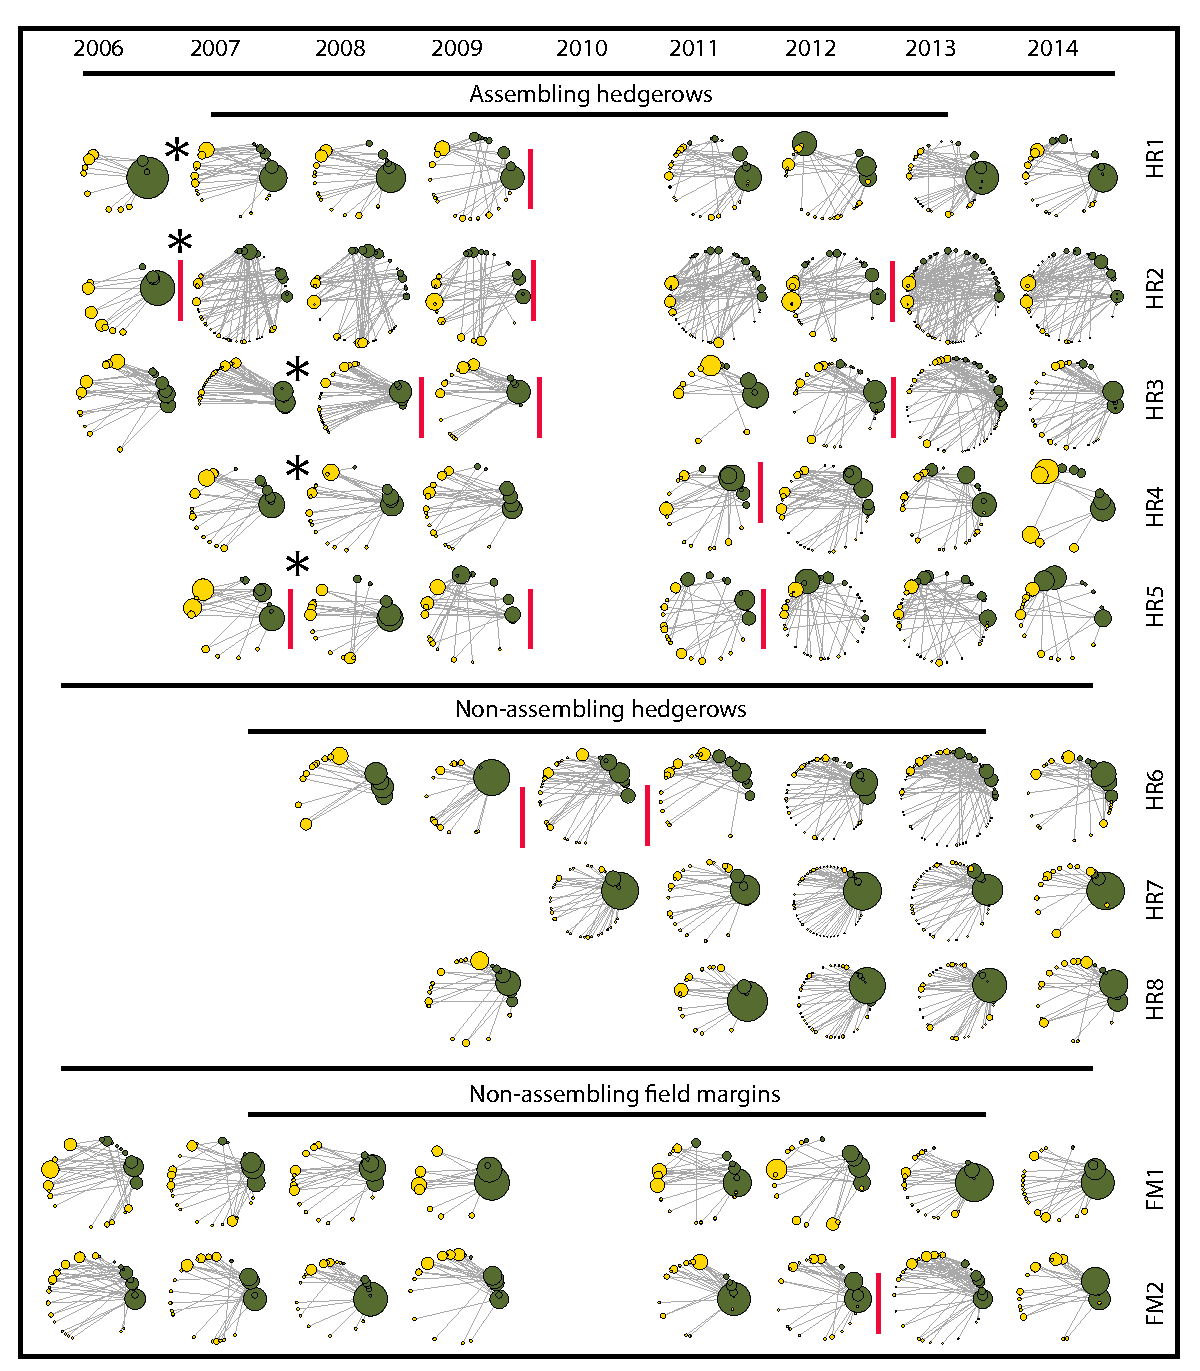
\includegraphics[width=1\textwidth]{../analysis/changePoint/plotting/networksv1.pdf}
  \caption{Assembling hedgerow networks had more changing points
    (vertical red lines) than non-assembling hedgerows and weedy field
    margins (a representative sample of non-assembling sites are
    depicted here). In each network, plants and pollinators are
    represented by green and yellow circles, respectively, weighted by
    their degree. Each species has a consistent position in the
    perimeter of the network across years. In the assembling
    hedgerows, colored squares in the corner of each network represent
    the year of assembly. Asterisks indicate the year the hegdgerow
    was planted. Before that, the sites were weedy field margins.}
  \label{fig:changePoints}
\end{figure}
\clearpage

\begin{figure}
  \centering
  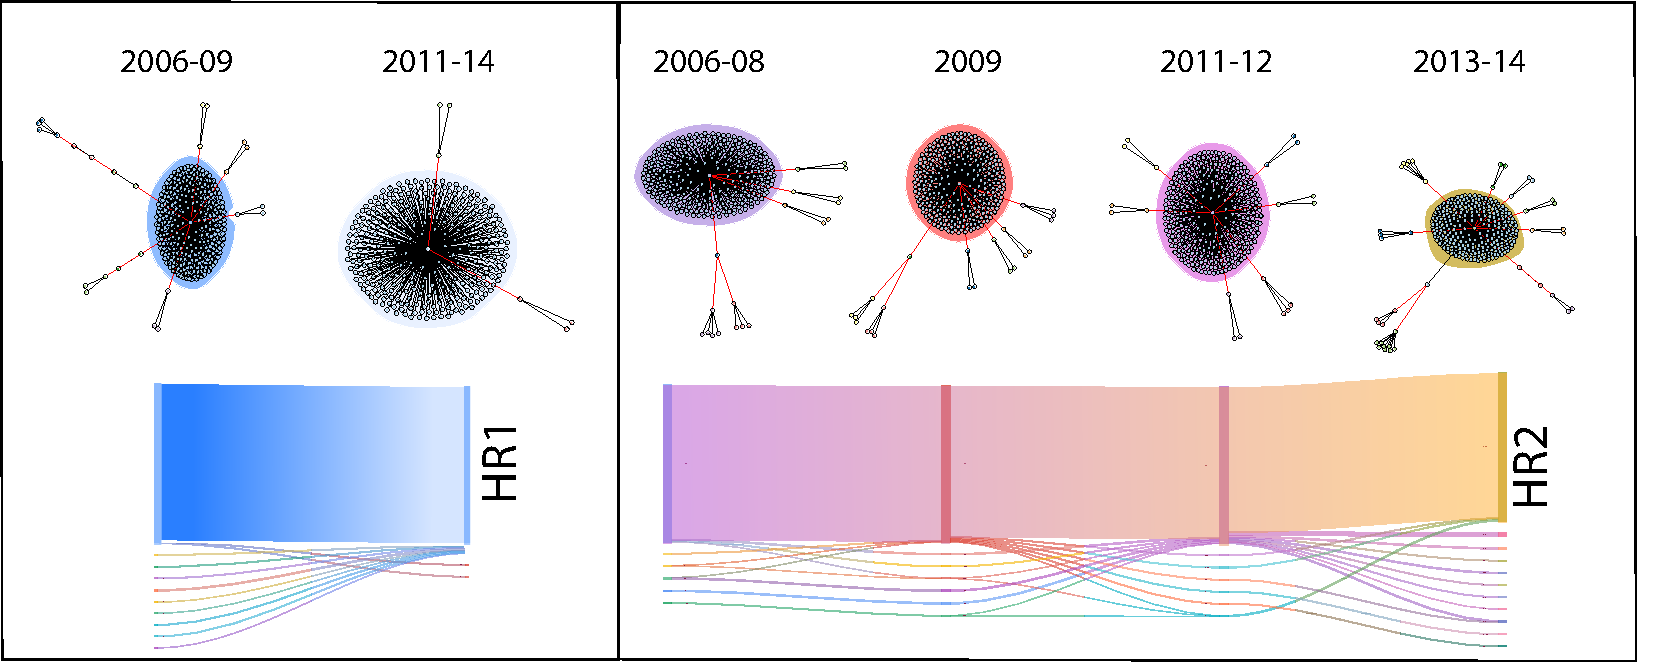
\includegraphics[width=.95\textwidth]{../analysis/changePoint/plotting/communitiesSkanky2.pdf}
  \caption{The module membership between network changing points. Two
    representative assembling hedgerows are depicted. In the top
    panel, species are grouped by community. The bottom panels
    visualize the flow of species between communities between changing
    points. }
  \label{fig:changePoints2}
\end{figure}
\clearpage

\begin{figure}
  \centering
  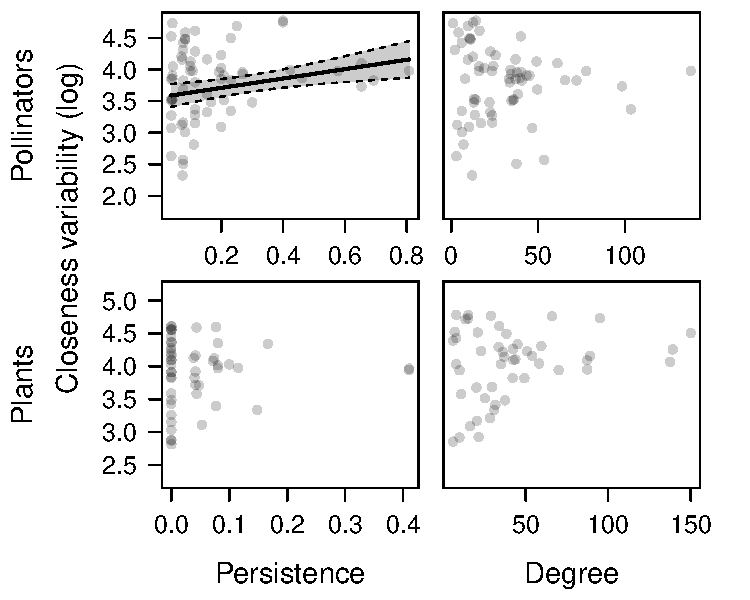
\includegraphics[width=.8\textwidth]{../analysis/variability/figures/cv/occ_degree.pdf}
  \caption{The variation coefficient of network position, as
    represented by closeness, plotted against pollinator persistence
    and degree. Persistence and degree were positively related to
    network position variability in pollinators, but unrelated in
    plants. Points represent means for each species across sites. The
    solid line indicates the mean slope estimate and the dashed lines
    are the $95\%$ confidence intervals around the estimate. }
  \label{fig:cv}
\end{figure}
\clearpage


\begin{figure}
  \centering
  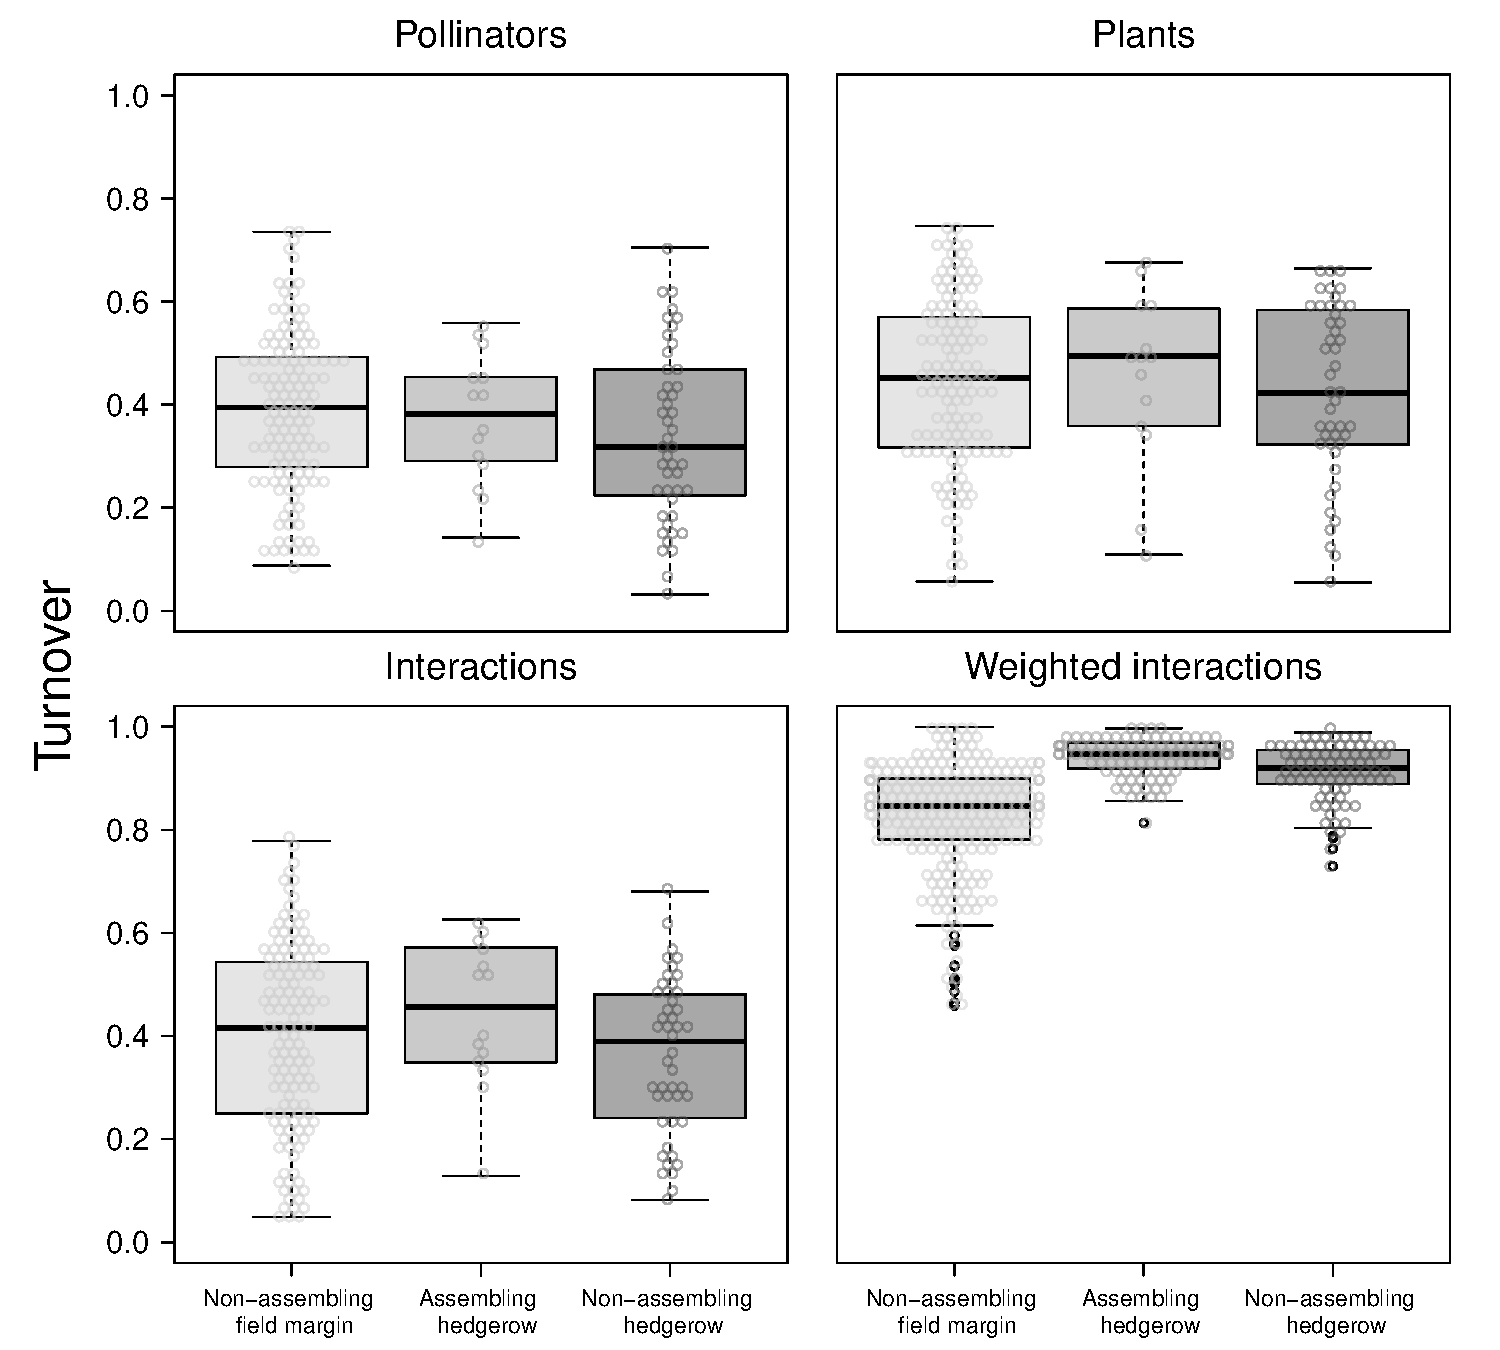
\includegraphics[width=1\textwidth]{../analysis/variability/figures/turnover_panels.pdf}
  \caption{The species, interaction and weighted interactions turnover
    of plant-pollinator networks at non-assembling field margins
    sites, assembling hedgerows, and non-assembling, mature
    hedgerows. Rates of species and interaction turnover were similar
    between site types, though mature hedgerows has marginally
    significantly less pollinator turnover.  However, when
    interactions where weighted by their similarity, both hedgerow
    types had higher turnover that unrestored field margins. Boxplots
    represent medians (black horizontal line) first and third
    quartiles (box perimeter) and extremes (whiskers). }
  \label{fig:beta}
\end{figure}
\clearpage



\begin{figure}
  \centering
  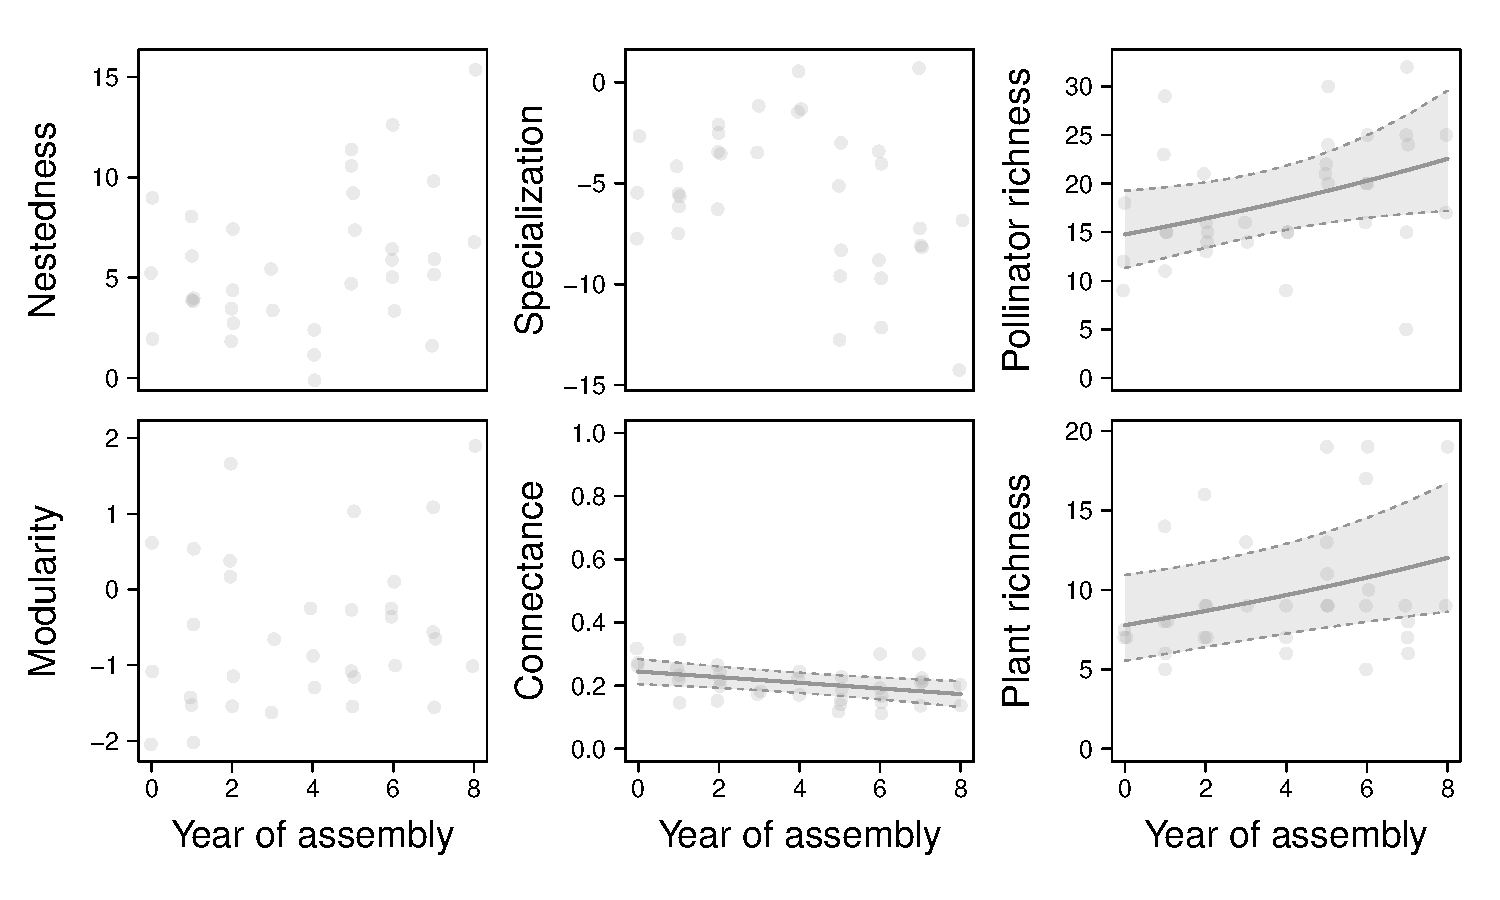
\includegraphics[width=1\textwidth]{../analysis/networkLevel/figures/baci.pdf}
  \caption{Nestedness, plant richness and pollinator richness
    increased as the networks assembled. Specialization and modularity
    remained consistent across years, while connectance decreased. The
    nestedness, modularity and specialization scores represent
    $z$-scores. Scores greater than $\sim 2$ or less than $\sim -2$
    are significantly more or less structured than randomly assembled
    networks. Points are the metric value for each site at each year
    of assembly. The solid line indicates the mean slope estimate and
    the dashed lines are the $95\%$ confidence intervals around the
    estimate.}
  \label{fig:baci}
\end{figure}
\clearpage


\begin{figure}
  \centering
  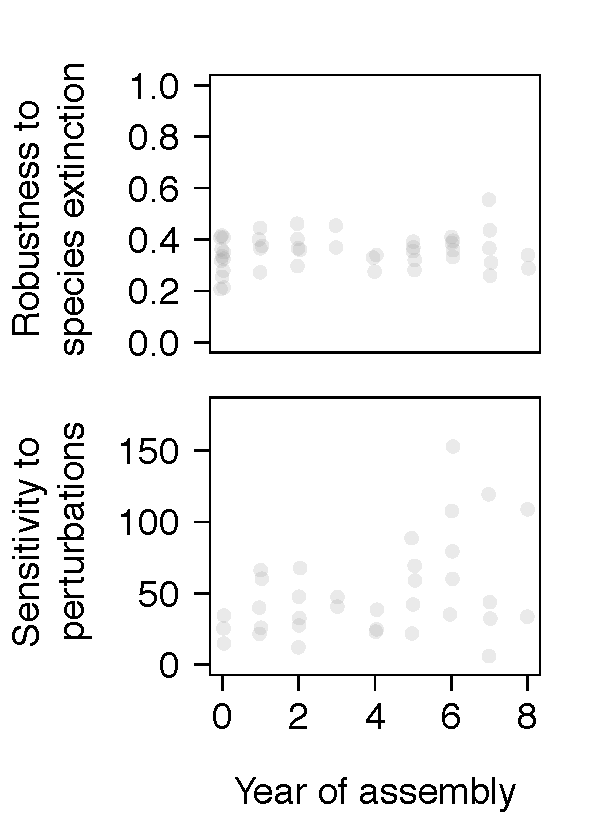
\includegraphics[width=.5\textwidth]{../analysis/networkLevel/figures/robustness.pdf}
  \caption{The robustness of networks to species extinction did not
    change with network assembly, but the sensitivity to cascading
    perturbations increased. The robustness to species extinction is
    measured by incrementally removing species by degree, though
    removing species by abundance did not yield qualitatively
    different results. The robustness of networks to cascading
    perturbations is measured as the algebraic connectivity, the
    second smallest eigenvalue of the Laplacian matrix. Points are the
    value for each site at each year of assembly. The solid line
    indicates the mean slope estimate and the dashed lines are the
    $95\%$ confidence intervals around the estimate.}
  \label{fig:rob}
\end{figure}
\clearpage

\end{document}

%%% Local Variables:
%%% mode: latex
%%% TeX-PDF-mode: t
%%% End:
